\documentclass[11pt]{report}
\usepackage{amsmath}
\usepackage{amsthm}
\usepackage{amssymb}
\usepackage{graphicx}
\usepackage{tikz}
\usepackage{multirow}
\usepackage{listings}
\usepackage{textcomp}
\usepackage{float}
\usepackage{subfig}
\usepackage[toc,page]{appendix}

\usepackage{listings}


\title{FARS : Functional Automated Reasoning System - v1.0}
\date{\today}
\author{Caner Derici}


\newtheorem{thm}{Theorem}
\newtheorem{prop}{Proposition}
\newtheorem{defn}{Definition}
\newtheorem{lemma}{Lemma}
\newcommand{\bra}[1]{\langle #1|}
\newcommand{\ket}[1]{|#1\rangle}
\newcommand{\braket}[2]{\langle #1|#2\rangle}
\newcommand{\cent}[0]{\mbox{\textcent}}
\newcommand{\dollar}[0]{\$}

\floatstyle{ruled}
\newfloat{algorithm}{htp}{lop}
\floatname{algorithm}{Algorithm}

\begin{document}
\pagenumbering{roman}

\maketitle
\tableofcontents



\chapter{General Overview}
\setcounter{page}{1}
\pagenumbering{arabic}

\paragraph{} FARS is a resolution-paramodulation style automated theorem prover, targeting first-order logic with equality. It's coded in Racket/PLAI language\footnote{For the details of these language, refer to Section ~\ref{section:plai}}. Its primary design goal is to be able to navigate very quickly in large search spaces and to cover a lot of space in a very short amount of time. Being coded in a functional style (although not purely functional) provides FARS to be highly modular in terms of heuristic usage and various compiler level optimizations that are accustomed to by many functional languages, such as tail call optimization.

\paragraph{} This document describes the current status of FARS, as well as serves as a documentation and a reference. Chapter 2 explains the theoretical concerns, such as the inference rules and heuristics used as well as the soundness and completeness. Chapter 3 describes the implementation and usage of FARS with as much example programs as possible. Chapter 4 shows several test runs with real theorems (which are given input to and solved by OTTER). Finally, Chapter 5 includes a discussion about the further development of FARS. Additionally, a complete reference of FARS can be found in Appendix A at the end of the document.

\chapter{Theoretical Perspective}

\section{General Characteristics}

\paragraph{} FARS is a resolution/paramodulation theorem prover which mainly employs the set of support strategy, along with hyperresolution, which is a special case of semantic resolution. It is designed to prove theorems expressed in first-order predicate logic with equality. Given the axioms and the negated conclusion as clauses\footnote{See Section~\ref{section:inputs} for more detailed discussion.}, FARS tries to prove it by resolution-refutation method. Furthermore, all of the proofs in FARS are refutations (by contradiction). 

\paragraph{} (REWRITE HERE) The main application areas of FARS in researches are generally abstract algebra and formal logic. It has been successful in answering many open questions in subfields of this sort, such as combinatory logic  and lattice theory .

% \paragraph{} Below are two example problems that can be easily answered by FARS:
% 
% \begin{itemize}
%  \item Prove that if a semigroup has a left identity with respect to which each element has a left inverse, then the semigroup is a group.\footnote{an exercise in group axiomatics}
%  \item A farmer has a wolf, a goat, and a basket of cabbages on the west bank of a river. The farmer also has a small boat, which beside himself can take not more than one of the wolf, the goat, and the cabbages. Given that he cannot leave the goat, or the goat alone with the cabbages, can the farmer transport himself, the wolf, the goat, and the cabbages to the east bank, and if so how?\footnote{The classical wolf, goat, and cabbages puzzle.}
% \end{itemize}
% 
% \paragraph{} The former problem is a simple theorem-proving problem, and solving it requires reasoning, however the latter one is a simple reasoning problem which requires a different reasoning strategy which would not normally be considered as an act of theorem proving. This happens to be the reason that FARS is commonly referred as an ``automated reasoning system''. 


\subsection{Inference Rules and General Strategy}

\paragraph{} The inference rules in FARS are generally based on resolution (with factorization) and paramodulation. In particular, FARS employs as inference rules binary resolution and hyperresolution. Additionally, equational deduction is done with binary paramodulation. Other attributes of FARS includes also forward and backward subsumption.

\section{Soundness \& Completeness}

\paragraph{} Generally, real automated reasoning systems (like OTTER) using resolution/paramodulation depend highly on search on huge spaces, thus they are implemented with numerous hacks and manual code-level optimizations. Therefore, it is highly impractical to prove something \emph{about} them. However, although a formal verification to any of the parts of the implementation of FARS has not been performed, its functional implementation allows a neat architecture for the system to be easily verified by automated verification systems. At this level, the output produced by FARS need to be manually checked by a human user.

\paragraph{} FARS's individual parts are designed and programmed to not affect the completeness of any of the theoretical aspects that is being implemented. Although some known weak points exist (see Section ~\ref{section:weak}), FARS completeness is established at a significantly desirable level. Full resolution is achieved by the repeated application of binary resolution, in where also the factorization is plugged. Forward and backward subsumptions are not affecting completeness. However, intentional constraints which affects the completeness for the sake of efficiency can be imposed manually, such as the \emph{max-step} parameter (which is false by default).

\section{Known Weak Points}                                                                                                                                                                                                                                                                                                                                                                                                                                                                                                                                                                                   
\label{section:weak}

\paragraph{} Due to the shortness of the implementation time, FARS include some known weak points that is to be solved in future versions to be developed. 

\paragraph{} One of the weak points is in the factorization. FARS's binary resolution adopt the idea that a clause can be inferred in four ways from its parents ($C_1$ \& $C_2$):

\begin{itemize}
 \item Resolution of $C_1$ and $C_2$
 \item Resolution of a factor of $C_1$ and $C_2$
 \item Resolution of $C_1$ and a factor of $C_2$
 \item Resolution of a factor of $C_1$ and a factor of $C_2$
\end{itemize}

Once FARS infer a resolvent from any of the possibilities above, it records $C_1$ and $C_2$ to what is called the \emph{main-memory}, and never try to resolve $C_1$ and $C_2$ again. This obviously ignores the possibility that more than one resolvents can be inferred from $C_1$ and $C_2$ that involves factorization, which in turn affect the completeness.

\section{Heuristics Used}

\paragraph{} FARS uses several heuristic approaches to different kinds of tasks, which are all governed by external heuristic functions provided as a parameter to the prover. This makes possible in future versions for heuristic functions to be provided even from the input files for individual theorems.

\paragraph{} Several points where a heuristic approach is being employed include:

\begin{itemize}
 \item Clause differentiation to generate nucleus and satellite for semantic resolution. Currently used built-in heuristic function implements hyperresolution by putting all the positive clauses to nucleus and all the others to satellite.
 \item Picking clauses from the set to be tried to resolve upon. Current heuristic chooses the clause with has the smallest number of literals.
 \item Predicate ordering to properly implement semantic resolution. Predicate ordering is automatically constructed from the given set of clauses by a heuristic function, again provided as input to the initiator. Current heuristic generates the ordering by putting the highest presedence to the mostly used predicate in the input. Additionally, by prove-for-all-pred-orders function, theorem can be tried to be proved by all possible permutations of the predicates one-by-one.
\end{itemize}


\chapter{Practical Perspective}

\paragraph{} FARS is written in Racket language using DrRacket environment. This chapter explains the general syntax and semantics of the Racket, as well as the basic usage of the DrRacket programming environment. The reason that the FARS is coded in Racket will be explained in the subseqent sections. At the most general view, FARS currently has 4 different purpose modules which have more than 1000 lines of codes in total. 

\section{Racket Language and DrRacket Environment}
\label{section:racketIntro}

\paragraph{} In Racket documentation, it is described informally as follows. 

\begin{quote}
Depending on how we look at it, Racket is

\begin{itemize}
 \item a programming language - a dialect of Lisp and a descendant of Scheme language;
 \item a family of programming languages - variants of Racket, and more; or
 \item a set of tools - for using a family of programming languages
\end{itemize}

\end{quote}

In this document, Racket is simply referred as a system of a general syntax (will be explained momentaily) and DrRacket environment. 

\paragraph{} Generally, Racket is a functional mainstream programming langauge, features (most importantly for us) first-class functions and tail-call optimization. Considering functions as first-class values, Racket provides a powerful programming framework, on which we can build theoretically the most general abstractions that could be created, such as function generating functions generating functions etc.

\paragraph{} Furthermore, Racket as a system, provides many programming langauges with different characteristics. FARS is built with the PLAI\footnote{Programming Langauge Application and Interpretation} langauge inside Racket, which is mainly used for studying the design and interpretation of programming langauge characteristics. The purpose of using particularly the PLAI language, is that the abstractions such as ``define-type'' and ``type-case'' are very useful in modeling and processing the statements of any formally representable language, such as first-order predicate logic in our case.

\paragraph{} The predominant disadvantage of using PLAI langauge is that it's evaluation is done via applicative order, which means a functions body is evaluated \emph{after} the arguments are evaluated first. When proving theorems, in many cases we do not perform anything on the whole data set, in other words, at each step there is at least one item which we don't touch. For example, consider the clauses choosen to be resolved upon from nucleus and satellite sets. Passing these sets as arguments to functions after functions, Racket evaluates all clauses within these sets although our algorithm doesn't touch them. Using a langauge that has a normal evaluation order in which the arguments are evaluated in a need basis would drastically improve the efficiency. 

\paragraph{} For more detailed overwiev of Racket language and DrRacket environment, as well as a list of built-in function explanations that will help understanding the implementation, please refer to Appendix~\ref{chapter:racket}.

\paragraph{} FARS is currently a non-interactive program. It reads its input from and writes the output to standard input and output respectively. It is ran on DrRacket. However, with the help of unix operators $<$ and $>$ which helps the files to interact with the standard i/o, it is possible for FARS to be modified easily such that it takes input from directly from the console, without using DrRacket. Currently all the options and parameters are given in the source file, but it is fairly easy to implement the necessary functionality to read parameters from individual theorem input files.

\section{Input \& Output}
\label{section:inputs}

\paragraph{} FARS accepts statements as disjuncted clauses, as all of FARS's inference rules and search algorithms operate on clauses.

\subsection{General Syntax and Naming}

\paragraph{} The general format of an input file to FARS is very simple. There can be comment lines, ``negated\_conclusion'' and the clauses. The clauses must be given in per line basis, i.e. there can be no clause seperated by a newline (\textbackslash n). Thus there is no need for the terms and statements to be terminated with periods. The propositional connectives such as ``not'' and ``or'' can be written with intuitive symbols such as ``-'' and ``$|$'' respectively.

\paragraph{} The output of FARS is divided into three parts. In the first part, FARS writes the input (without the comments) with the clauses augmented with their identification number and predicate counts. If the \textit{starter-verbose} flag is set to be true, the second part where the individual search steps (involving resolvents and factorizations) are produced as the search goes on. Finally if FARS found a proof, it produces a human readable proof which can be traced and checked easily.

\paragraph{} Following is a simple theorem from TGTP;

\lstset{
    literate={~} {$\sim$}{1},basicstyle=\small
}

\begin{lstlisting}
; A.THM  See TGTP, Chapter 6, Section 6.1
P(x) | ~Q(x)

Q(a()) | Q(b())
 
negated_conclusion
~P(x) 
\end{lstlisting}

\paragraph{} When the above example input is given to FARS, it easily finds the solution and outputs as follows:

\begin{lstlisting}
Initiating the input : 
<ID> <predCount> <actualClause>
(1 2 (P(x) ~Q(x)))
(2 2 (Q(a) Q(b)))
(3 1 (~P(x)))


Initial predicate order: 
(Q P)



proof-found! unit conflict.

From 1 and 2, generate -> 4 - P(b) | Q(a)

From 3 and 4, generate -> 5 - Q(a)

From 1 and 5, generate -> 6 - P(a)

From 6 and 3 ---> F
'proof-found!
\end{lstlisting}

\subsection{Restrictions in Input}

\paragraph{} Current version of FARS impose some restrictions for the format in input files. These restrictions are:

\begin{itemize}
 \item There can be no whitespaces among the arguments of a predicate or a function, i.e. anywhere between ( and ).
 \item There can be no predicates without a variable, so inputs such as 

A $|$ B should be turned into A(x) $|$ B(x).
 \item There can be no tab (\textbackslash t) characters
 \item Comment symbol (;) must be at the beginning of the line. inputs like 

A $|$ B ; axiom 6

are not permitted.
 \item Variable or constant symbols should be one letter. 
\end{itemize}

\paragraph{} These restrictions are to be fixed in further versions of FARS.


\subsection{Naming}

\paragraph{} FARS has a simple naming characteristic. If a simple term occurs in a clause, the default behavior is to look at the symbol to decide its type. If it starts with \emph{x,y,z,g,t,u,v}, then it is classified as a variable, and if starts with \emph{a,b,c,d,e}, it is classified as a constant.

\section{The Main Loop}
\label{section:mainloop}

\paragraph{} FARS's primary inference mechanism is semantic resolution. Current clause differentiator generates the nucleus and satellite sets by being positive or mixed, just as in hyperresolution, however, this can be easily modified since the differentiator function is provided as a parameter to the prover. 

\paragraph{} As mentioned before, FARS operates on mainly two different sets called nucleus and satellite, which by default contains all positive and mixed clauses respectively. The algorithm is as follows: \newline

\hrule \vspace{2mm}
While (proof-nucleus-memory not contains all of nucleus clauses and no refutation has been found)
\begin{enumerate}
 \item Let \textit{nuc\_clause} be the ``best'' clause in nucleus
 \item Choose a suitable \textit{sat\_clause} from satellite which contains a negated version of a predicate of \textit{nuc\_clause}
 \item Infer the \textit{new\_clause} using binary resolution and factorization. 
 \item Merge identical literals and apply factor-simplification
 \item If \textit{new\_clause} has 0 literals, a refutation has been found, stop and initiate the proof printing sequence.
 \item If max-literals parameter is set, check the number of literals and discard \textit{new\_clause} if there are too many
 \item If \textit{new\_clause} is a unit clause, check for unit conflicts
 \item Put \textit{new\_clause} to nucleus if it is a positive clause, otherwise, put it to satellite
\end{enumerate}

\hrule

\chapter{Test Drive}

\paragraph{} In this section, we run FARS on 4 different theorems with somewhat similar characteristics. We provide both the input and output and give (although not line-by-line) a small comment on the problem.

\section{Pigeon Hole Problem}

\paragraph{} The first example is the famous ``Pigeon Hole Problem'', stated as axioms and a negated conclusion. This particular instance of the problem involves 5 pigeons and 4 holes, and FARS proves that one pigeon must have been left out. Below are the input and the output produced by FARS.

\lstset{
xleftmargin=-55pt
}

\lstinputlisting[basicstyle=\scriptsize]{pigeon.THM}

\paragraph{} FARS output:

\lstinputlisting[basicstyle=\scriptsize]{pigeon.out}


\section{Lifschitz's theorem}

\paragraph{} This example demonstrates the use of prove-file-preds which tries to prove the theorem with all possible permutations of the predicate order. Note that starter-verbose flag is set to be false, thus the intermediate search steps are not included in the output.

\paragraph{} The proof is as follows:

\lstset{
xleftmargin=-55pt
}

\lstinputlisting[basicstyle=\scriptsize]{LIFSCHTZ.THM}

\paragraph{} FARS output:

\lstinputlisting[basicstyle=\scriptsize]{lifschtz.out}

\newpage

\section{LINEAR}

\paragraph{} Again, using the prove-file-preds to try all the predicate orders.

\lstset{
xleftmargin=-55pt
}

\lstinputlisting[basicstyle=\scriptsize]{LINEAR.THM}

\paragraph{} FARS output:

\lstinputlisting[basicstyle=\scriptsize]{linear.out}



\section{The Lion and the Unicorn Puzzle}

\paragraph{} This example basically shows that FARS is not only a theorem prover, but an automated reasoning system, which can be used to solve mathematical puzzles, stated as axioms and conclusion. This puzzle is from Alice in Wonderland as follows:

\begin{quote}
 When Alice entered the forest of forgetfulness, she did not forget everything, only certain things. She often forgot her name, and the most likely thing for her to forget was the day of the week. Now, the lion and the unicorn were frequent visitors to this forest. These two are strange creatures. The lion lies on Mondays, Tuesdays, and Wednesdays, and tell the truth on the other days of the week. The unicorn, on the other hand, lies on Thursdays, Fridays, and Saturdays, but tells the truth on the other days of the week.

One day Alice met the lion and the unicorn resting under a tree.  They made the following statements:

Lion:  Yesterday was one of my lying days.

Unicorn:  Yesterday was one of my lying days.

From these statements, Alice, who was a bright girl, was able to deduce the day of the week.  What was it?
\end{quote}


\paragraph{} The proof that today is actually Thursday, is as follows (again the verbosity is disabled due to space concerns):

\lstset{
xleftmargin=-55pt
}

\lstinputlisting[basicstyle=\scriptsize]{LION.THM}

\paragraph{} FARS output:

\lstinputlisting[basicstyle=\scriptsize]{lion.out}


\chapter{Discussion and Future Work}

\paragraph{} There are currently lots of deficiencies and inefficiencies in FARS due to time concerns. These are planned to be improved or corrected in the future versions. Below are explanations for each planned future work:

\begin{itemize}
 \item The known full completeness issue due to the factorization is to be corrected.
 \item The efficiency of the whole system can be drastically improved by incorporating FARS to a platform with normal order evaluation strategy (such as lazy racket).
 \item Unit testing as well as an overall performance testing is required. Possibly a helper module implementing the necessary functionality for test functions to be generated and applied for other modules to be able to test themselves easily. This way, comprehensive test suite can be automatically generated, which is a huge step in validating the soundness and correctness of the whole system.
 \item FARS is currently working in a non-interactive mode. Proof searching should be interruptable, as well as continuable after certain parameters are modified in between. This functionality obviously require FARS to be able to run in interactive mode.
 \item The restrictions in the format of the input files should be released.
 \item FARS is highly generalized, as all the heuristics and even some parts of its inference strategy can be provided as a parameter. This can be further improved by supporting these parametizations at the input file level, where for example heuristic functions to be used are directly fed from the input file.
 \item An advanced weighting system and also the ``hints strategy'' can be adopted from OTTER, which are very useful for the core prover to navigate in the search space very efficiently.
 \item A better improvement for heuristic usage is to implement the necessary framework for supporting the learning heuristics, which employ machine learning techniques to learn and improve themselves for the similar proof tasks.
\end{itemize}

\paragraph{} At the current stage, FARS can not perform well on a very broad area of theorems, however, its efficiency in proving is clearly observable despite the inefficient parts of its implementation. It's functional and generalized characteristics on the other hand, provides that FARS can be made to be very capable prover with a very little effort.

\begin{appendices}
 \chapter{Complete Reference}

\paragraph{} Below are the sections involving explanations for each and every part of the implementation. This reference is designed to be a direct informal reflection of the implementation. Thus the reference is \textbf{not} alphabetical, but spatial with respect to the implementation. It can be referred by using the context of the item or the part in consideration. For example, section names are actually source file names, and each section contains all global parameters as well as functions in the order that they are appearing in the actual source.

\paragraph{} Functions include contracts beside their names. For example

\begin{itemize}
 \item \textbf{factor} : clause -$>$ clause
\end{itemize}

means that the function named \textit{factor} consumes a single clause and produces a single clause. Higher arities are indicated by a single space break between input parameters in the contract.

\begin{itemize}
 \item \textbf{resolve} : clause clause (listof symbol?) -$>$ clause
\end{itemize}

meaning that the function named \textit{resolve} consumes two clauses and a list of symbol (indicating the predicate order) and produce a single clause (resolvent).

\paragraph{} Function contracts are not an explanation of what a function does, but only an indicator of input-output relationships in order to ease the functional development process.

\newpage

\section{Main}

\subsection{Global Parameters}

\begin{itemize}
 \item \textbf{max-step}
 
A run-time constraint parameter. Limits the maximum steps taken by the prover. Default to false.

 \item \textbf{max-literal}

A simple heuristic for resolution. Any inferred clause that is bigger than the \textit{max-literal} parameter is discarded.

 \item \textbf{verbose}

 Verbosity flag. Can either be true or false.

 \item \textbf{starter-verbose}

 Sometimes the prover can set its verbosity level itself, \textit{starter-verbose} is used to reset the \textit{verbose} flag. Mostly used in subsequent automatic runs of the FARS.

 \item \textbf{init}

 An internal flag controlling the repeated application of \textit{binary-resolution}. When \textit{binary-resolution} returns false, \textit{resolve} understands from \textit{init} whether the given clauses are originally not resolvable or not further resolvable. Defaults to true.

 \item \textbf{last-input-index}

 A mutable parameter that is set by the \textit{initiate} function, indicating the ID of the last clause given in input. Used by \textit{print-proof}.

 \item \textbf{main-memory}

A list containing pairs of clause ID's (e.g. (4 12)) that are used by the resolution. Each time a new clause is inferred, its parents are recorded to \textit{main-memory} in order to avoid duplicate resolutions.

 \item \textbf{proof-nucleus-memory}

A list containing the ID's of the clauses from nucleus that is failed to be of any use with that particular stage of the prover. Each time a new clause inferred, \textit{proof-nucleus-memory} is reset to be empty, so that previous nucleus clauses can be tried with new clauses.

 \item \textbf{proof-memory}

A list containing a lot of information about each semantic clash, helping the proofs to be printed easily. Each time a proof is found, \textit{proof-memory} is scanned backwards from the top of the \textit{main-memory} to construct a step-by-step human readable proof.
\end{itemize}

\subsection{Functions}

\begin{itemize}
 \item \textbf{factor} : clause -$>$ clause

Implements full factorization by repeatedly applying itself, corresponding to a repeated application of binary factorization.

 \item \textbf{resolve} : clause clause (listof symbol?) -$>$ clause

Just a wrapper function to initiate correctly the resolution parameters before the resolution begins.

 \item \textbf{resolve-inner} : clause clause (listof symbol?) -$>$ clause

Like \textit{factor}, it implements full resolution by repeatedly calls itself, which is actually performing binary resolution. Note that, \textit{resolve-inner} tries to resolve the factorizations of the given clauses as well as the clauses themselves. Whenever it finds a single resolvent, it stops to try others and goes on with that resolvent.

 \item \textbf{binary-resolve} : clause clause (listof symbol?) -$>$ (listof clause clause)

Implements binary resolution on given two clauses, considering the given predicate ordering. It does not return a single resolvent clause, but returns two clauses that are ready to form the resolvent by simply appending together. The reason is to easily repeat the binary-resolution on them to perform full resolution.

 \item \textbf{initiate} : (listof clause) pred-order-constructor clause-differentiator clause-picker -$>$ prover-input-object

Constructs a \textit{pi} object to be consumed by the prover. Indexes the given clauses, construct the predicate order by the given pred-order-constructor, differentiate nucleus and satellite sets by the given clause-differentiator and puts all of the initial information that is needed by the prover in the \textit{pi} object.

 \item \textbf{struct:pi}

PI (prover-input) is a structure containing all the necessary parameters to initiate the prover, such as nucleus and satellite sets, unit clauses, clause picker function and predicate order.

 \item \textbf{start} pi-object -$>$ proof

Just a wrapper function to set the global parameters and run the prover with the given pi-object.

 \item \textbf{easy-init} : (listof clauses) -$>$ proof

We have built-in predicate ordering, nucleus/satellite differentiator (interpretation creator) and clause picker functions. \textit{Easy-init} is a wrapper for these built-in functions to call \textit{initiate} easily with them.

 \item \textbf{prove-file} : string? -$>$ proof

Just a wrapper function to parse the given file-name, run \textit{easy-init} and then \textit{start}.

 \item \textbf{prove} : nucleus satellite nuc-units sat-units clause-picker pred-order next-index step -$>$ proof

Implements the main prover loop. \textit{next-index} is used to index the newly inferred clause. \textit{step} counts the number of steps the prover takes, mainly for using \textit{max-step} control. Detailed discussion about the implemented algorithm can be found in Section ~\ref{section:mainloop}.

 \item \textbf{sieve-clause-set} : (listof siever-functions) (listof clause) chosen-nuc-clause-ID -$>$ (listof clause)

Mainly used in satellite clause selection. \textit{sieve-clause-set} eliminates the irrelevant clauses in satellite set according to the given list of eliminator functions constructed using the chosen nucleus predicates. These functions together decide whether a clause in satellite is suitable or not for the chosen clause in nucleus, by looking at its literals.

 \item \textbf{unit-conflict-check} : clause (listof clause) (listof symbol?) -$>$ proof

Performs the widely-known unit conflict check. Each time a unit clause is inferred in \textit{prove}, \textit{unit-conflict-check} is run to find an easy proof quickly. 

 \item \textbf{start-with-order} : (listof symbol?) pi-object -$>$ proof

Just another helper function for \textit{prove}. Essential purpose is to make possible to override the predicate order constructor function and provide a particular order manually.

 \item \textbf{start-for-all-preds} : pi-object -$>$ proof

Like \textit{start} for \textit{prove}, \textit{start-for-all-preds} is just a wrapper function to set the global parameters and run the \textit{prove-for-all-pred-orders} with the given pi-object.

 \item \textbf{prove-for-all-pred-orders} : pi-object (listof (listof symbol?)) -$>$ proof

When a suitable predicate order constructor function can not be found, \textit{prove-for-all-pred-orders} generates all possible permutations of the predicates and tries to prove them one by one normally.

 \item \textbf{prove-file-preds} : string? -$>$ proof

Like prove-file, a wrapper function to parse the given file-name, run \textit{easy-init} and then \textit{start-for-all-preds}.

 \item \textbf{print-proof} : (listof clause?) proof-memory -$>$ (void)

Just prints the proof sequence constructed by the construct-proof-sequence using proof-memory. Returns nothing.

 \item \textbf{print-real-proof} : proof-sequence -$>$ (void)

This consumes the proof-sequence generated by the construct-proof-sequence and displays them in a human readable format one by one. Returns nothing.

\end{itemize}

\section{Util}

\subsection{Functions}

\begin{itemize}
 \item \textbf{extract-args} : string? -$>$ (listof string?)

A wrapper function for \textit{extract-arguments}.

 \item \textbf{comma-after-paren-count0} : (listof char?) number number -$>$ number

A helper function for extract arguments, to handle situtations like f(\ \ x(),g(h(),p())\ \ ). Returns the comma index after the balanced paranthesis.

 \item \textbf{extract-arguments} : string? output-list -$>$ (listof string?)

Extracts the comma seperated strings as a list from the given string. output-list is just for implementing tail-recursion.

 \item \textbf{remove-identicals} : clause -$>$ clause

Removes all the identical literals in the given clause.

 \item \textbf{disagreement-dive} : clause -$>$ clause

A helper function for \textit{disagreement-set}. Essentially a hack to handle the cases such as f(g(k)) f(u) --$>$ \{g(k),u\}. 

 \item \textbf{disagreement-set} : (listof (listof FOP?)) -$>$ (listof FOP?)

Extracts the disagreement set from the given argument set of literals

 \item \textbf{preliminary-check} : (listof clause?) -$>$ boolean

A helper for \textit{unify} to check if the given list of clauses all contain the same predicate names and parameter numbers. If not, unification can stop immediately without computing anything.

 \item \textbf{find-term} : var? (listof FOP?) -$>$ FOP?

Finds the first term in the disagreement set that not includes the given variable. Essentially a helper for \textit{find-var-term} to find a term.

 \item \textbf{find-var-term} : (listof FOP?) -$>$ (listof var? FOP?)

Extracts a \{v/t\} pair from the given disagreement set. Essentially a helper for \textit{unify}.

 \item \textbf{apply-subst} : (listof var? FOP?) clause -$>$ clause

A helper function for \textit{apply-mgu}. Applies a single substitution to the given clause.

 \item \textbf{apply-mgu} : (listof (listof var? FOP?)) clause -$>$ clause

Applies the given set of substitutions to the given clause, using \textit{apply-subst} repeatedly.

 \item \textbf{unify} : (listof clause?) (listof (listof var? FOP?)) -$>$ (listof (listof var? FOP?))

Implements the unification algorithm on the given set of clauses to produce a most general unifier (set of substitutions). The second parameter is merely to implement tail-recursion.

 \item \textbf{find-unifiable-pair-mgu} : clause clause -$>$ (listof mgu clause clause)

Finds a unifiable pair of terms from the given clauses and produce their mgu's along with the chosen clauses.

 \item \textbf{fup-mgu/factor} : clause clause -$>$ (listof mgu clause clause)

Like find-unifiable-pair-mgu, but ignores that the choosen terms are exactly the same. Mostly used in factorization for finding a unifiable pair of terms in the same clause.

 \item \textbf{detach-literal} : FOP? clause -$>$ clause

Detaches the given literal from the given clause. Mostly used in resolution, to detach the resolved literals.

 \item \textbf{pred-or-neg-with-name} : symbol? -$>$ (FOP? -$>$ boolean?)

Constructs a function which consumes a literal (pred or negated pred) and checks if it has the name which is originally a parameter to \textit{pred-or-neg-with-name}.

 \item \textbf{pred-with-name} : symbol? -$>$ (FOP? -$>$ boolean?)

Like \textit{pred-or-neg-with-name}, but only checks for non-negated predicates.

 \item \textbf{neg-with-name} : symbol? -$>$ (FOP? -$>$ boolean?)

Converse of \textit{pred-with-name}, only checks for the negated predicates.

 \item \textbf{contains-pred-or-neg} : clause symbol? -$>$ boolean?

Checks if the given clause contains the predicate or its negation with the given name.

 \item \textbf{highest-pred-in} : clause (listof symbol?) -$>$ symbol?

Produces the name of the predicate that has the highest order in the given clause.

 \item \textbf{rename-vars} : clause clause -$>$ (listof clause clause)

If the given clauses have variables with the same names, it systematically renames the shared variables in one of the clauses with automatically generated unique variable names.

 \item \textbf{process-same-lits} : clause clause -$>$ (listof clause clause)

This is essentially a hack. It constructs an artificial mgu and applies it to one of the clauses that will make possible EXACTLY SAME (negated) literals to be resolved by the normal resolution procedure. Consider c1:P(x)VQ(x) and c2:\~P(x)V\~Q(x). Normally c1 will be renamed like P(gsymb1)VQ(gsymb1), thus the resolution does not resolve these literals with literals in c2 (since P(x) and \~P(y) are not unifiable). However, \textit{process-same-lits} turn c1 into P(a)VQ(a) and do not touch c2. Therefore, resolution will be forced to resolve these.

 \item \textbf{construct-inner-mgu} : clause clause (listof (listof var? FOP?)) -$>$ (listof (listof var? FOP?))

Actual worker function in \textit{process-same-lits}, constructing the necessary mgu.

 \item \textbf{choose-unifiable-literals} : clause clause (listof symbol?) boolean -$>$ (list mgu FOP? FOP?)

Chooses two literals L1 and L2 from C1 and C2 respectively, according to the given predicate order, such that L1 and \~L2 are unifiable. Note that hack-flag (the last parameter) is used for ignoring the predicate order, generalizing the function further.

 \item \textbf{count-preds} : FOP? number -$>$ number

Counts the number of predicates in the given literal. Second parameter is only for tail-recursion.

 \item \textbf{count-preds-clause} : clause -$>$ number

Counts the number of predicates in the given clause, using \textit{count-preds}.

 \item \textbf{construct-pred-order} : (listof clause) -$>$ (listof symbol?)

This is an example predicate order constructor function. It consumes a set of clauses and produces a predicate order such that the first predicate in the output has the highest number of occurance in the set. 

A lot of predicate order constructor functions can be created and provided to the prover as input. \textit{construct-pred-order} is only an example.

 \item \textbf{picker-example} : (listof (listof number number clause)) -$>$ (listof number number clause)

This is an example clause picker for tasks like resolution where a clause need to be picked from the set of clauses. \textit{picker-example} chooses the clause with the least predicate count.

 \item \textbf{differentiator-example} : (listof (listof clauses)) -$>$ (listof (listof clauses) (listof clauses))

This is an example differentiator function, extracts the nucleus and satellite sets of clauses by putting all positive clauses to nucleus, and mixed ones into the satellite.

 \item \textbf{insert-everywhere} : any (listof any) (listof any) (listof any) -$>$ (listof (listof any))

A helper function for \textit{generate-all-permutations-of}. Inserts the given element into every possible places among the elements in the third argument. The second and fourth arguments are for tail-recursion. Example usage: (insert-everywhere 2 '() '(1 3) '()) will produce '((2 1 3) (1 2 3) (1 3 2))

 \item \textbf{generate-all-permutations-of} : (listof any) -$>$ (listof (listof any))

Produce all possible permutations of the given list of elements. Mostly used by \textit{prove-for-all-pred-orders}.

 \item \textbf{construct-proof-sequence} : proof-memory (list id id) id -$>$ (listof (listof id id (id clause)))

A helper for \textit{print-proof}. Constructs the proof-sequence of the found proof by backtracking in proof-memory, starting from the given end-point (second parameter).

\end{itemize}

\section{Language}

\subsection{Global Parameters}

\begin{itemize}
 \item \textbf{constant-symbols}

This list constitute the symbols mostly used for constants in input theorems. By default, it contains \{a,b,c,d,e\}.

 \item \textbf{var-symbols}

Like constant-symbols, but for variable symbols. By default, it contains \{x,y,z,g,t,u,v\}.
\end{itemize}

\subsection{Functions}

\begin{itemize}
 \item \textbf{constant?} : symbol? -$>$ boolean?

Checks if the given symbol is among constant symbols or not in variable symbols.

 \item \textbf{variable?} : symbol? -$>$ boolean?

Checks if the given symbol is among variable symbols or not in constant symbols.

 \item \textbf{listof?} : (any -$>$ boolean?) -$>$ ((listof any) -$>$ boolean?)

Constructs a function which will consume a list of elements and apply the given predicate function to every element of the list, checking every element satisfies the predicate.

 \item \textbf{FOP}

This is not a function, but a data type, representing a single term. 

 \item \textbf{FOP=?} : FOP? FOP? -$>$ boolean?

Checks if the given two terms are exactly the same.

 \item \textbf{var-contain?} : var? FOP? -$>$ boolean?

Checks if the given term contains the given variable.

 \item \textbf{rewrite-term} : var? FOP? FOP? -$>$ FOP?

Substitutes the given variable with the given term(second parameter) in the third parameter.

 \item \textbf{var-names} : clause (listof symbol?) -$>$ (listof symbol?)

Extracts the variable names from the given clause. Second parameter is for tail-recursion.

 \item \textbf{pred-names} : clause (listof symbol?) -$>$ (listof symbol?)

Like \textit{var-names}, but for predicate names.

 \item \textbf{neg-pred-names} : clause (listof symbol?) -$>$ (listof symbol?)

Like \textit{var-names}, but for negated predicate names.

 \item \textbf{extract-names} : (clause-$>$(listof symbol?)) clause -$>$ (listof symbol?)

Extracts the names using the given function from the given clause.

 \item \textbf{extract-names-from-S} : (clause-$>$(listof symbol?)) (listof clause) -$>$ (listof symbol?)

Extracts the names using the given function and \textit{extract-names} from the given set of clauses.

 \item \textbf{process-args} : (listof FOP?) string? string -$>$ string

Helper function for \textit{unparse} to place seperators between the unparsed arguments.

 \item \textbf{unparse} : FOP? -$>$ string?

Unparses the given term.

 \item \textbf{unparse-clause} : clause -$>$ string?

Unparses the given clause using \textit{unparse}.

 \item \textbf{unparse-S} : (listof clause?) -$>$ string?

Unparses the given set of clauses using \textit{unparse-clause}.
\end{itemize}

\section{Parser}

\subsection{Global Parameters}

\begin{itemize}
 \item \textbf{comment}

Comment symbol used to indicate a comment line in the given input. Defaults to ``;''.

 \item \textbf{negline}

String used to indicate the negated conclusion in the input. Defaults to ``negated\_conclusion''.

 \item \textbf{or-sym}

String used to indicate the disjunction in the given input. Defaults to ``$|$''.

 \item \textbf{or-char}

Like or-sym, but in type char. Defaults to ``$\# \backslash |$''.
\end{itemize}

\subsection{Functions}

\begin{itemize}
 \item \textbf{pre-process} : (listof (listof string?)) -$>$ (listof (listof string?))

Performs the pre-processing tasks like empty line, comment line and ``negated\_conclusion'' deletion before parsing begins.

 \item \textbf{remove-or-symbols} : (listof string?) -$>$ (listof string?)

Removes the \textit{or-sym}'s from the unparsed lines.

 \item \textbf{parse-term} : string? -$>$ FOP?

Parses a single unit of the given input theorem. Assumptions about the input file include (-) function-like symbols with no arguments are actually constants (like a()), and (-) there are no nested predicates.

 \item \textbf{parse-term-inner} : boolean? string -$>$ FOP?

Actual working function withing \textit{parse-term}. The first argument indicates whether we dove into the parameters of a predicate, or we are at the top level (false means we are looking for a predicate, true means a function).

 \item \textbf{parse-clause} : (listof string?) -$>$ clause

Parses the given clause line using \textit{parse-term}.

 \item \textbf{parse-file} : symbol? -$>$ (listof clauses)

Parses the given file using \textit{read-words/line}(from Racket library), \textit{pre-process} and \textit{parse-clause}, producing the raw set of clauses to be initialized and proved.

\end{itemize}

\chapter{Racket as a System}
\label{chapter:racket}

As briefly explained in Section~\ref{section:racketIntro}, Racket is a rather big system containing a lot of programming languages, an advanced programming environment, as well as lots of different kinds of tools in it. In this chapter, we try to provide a general idea about the syntax and semantics of the Racket language and DrRacket environment, which will hopefully be helpful in understanding the implementation of FARS.

\section{Overview of Syntax and Semantics}
\label{section:plai}

\paragraph{} Almost all of the dialects of LISP including Racket uses s-expressions as a concrete syntax. The self referential definition of s-expressions is as follows:

An s-expression is:
\begin{itemize}
 \item an atom (mostly indicated by a symbol), or
 \item a list of of s-expressions
\end{itemize}

For instance, a, (), (a), ((a)) or (a (b (c) (d)) (((e)))), are all s-expressions. Note that however, all Racket expressions are s-expressions, but not all s-expressions are Racket expressions.

\paragraph{} In particular, Racket uses s-expressions in a prefix form, in which the functions and operators are written \emph{before} arguments, such as

(+ 1 2)

or

(prove-file ``LION.THM'')

\paragraph{} Every definition in Racket uses (define ...) structure. Because the functions are treated as first-class values (like numbers), they are also defined in this way.

(define a 5)

(define (sqr x) (* x x))

\paragraph{} As explained in the previous paragraphs, a defined function is applied in again the prefix way, such as

(sqr 5)

\section{DrRacket}

\paragraph{} DrRacket is an interactive programming environment, which involves two main frames as can be seen in the following figure.

\begin{center}
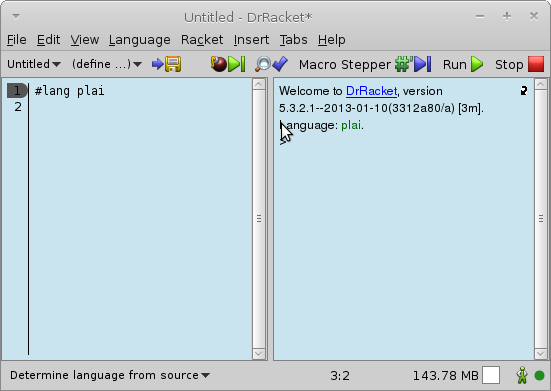
\includegraphics[scale=0.75]{DrracketMain.png}
\end{center}

\paragraph{} Two main frames are called the ``definitions'' (left in the figure) and ``interactions'' (right in the figure) windows. The program definitions are written in the definitions window and when the ``Run'' button is pressed, the definitions are parsed and compiled automatically, at which point the interactions window can be used to run the programs manually or automatically.

\paragraph{} The interactions window implements what is called the REPL (Read-Eval-Print Loop), in which the programs are read, evaulated, the corresponding outputs are written and then the reading starts again and so on. It can be considered as a very complicated calculator, on which we can run arithmetic expressions as well as prove theorems, given that the necessary definitions are provided. At default settings, the interaction window also serves as the standard output which is exactly the same thing that we know from various other contexts such as Linux console. In fact, the programs written in DrRacket can also be computed through the console program ``racket'', passing the outputs to the real standard output.

\paragraph{} DrRacket can be run on all mainstream platforms such as Linux, Mac OS and Windows. It can be downloaded from:

\begin{center}
 http://download.racket-lang.org/
\end{center}

The complete documentation of the Racket system can be found at:

\begin{center}
 http://docs.racket-lang.org/
\end{center}

\section{Some Built-In Racket Functions}

\paragraph{} In this section, we try to explain several built-in functions of Racket that is used to implement FARS, along with examples where necessary. Most of the functions described below are list processing functions, because Racket is a not so long cousin of LISP (list-processing) language. Thus, it would be appropriate to give a formal definition of a list of elements.

A listof elements is either:
\begin{itemize}
 \item empty, or
 \item (cons e ls), where e is an element and ls is a listof elements.
\end{itemize}

\paragraph{} Here are the built-in Racket functions which are most frequently used in the implementation of FARS.

\begin{itemize}
 \item \textbf{cons} : constructs a list from the given two arguments.

(cons 4 empty) -$>$ (4)

(cons 4 (cons 6 empty)) -$>$ (4 6)

 \item \textbf{car} : extracts the first element of the given list.

(car (cons 3 empty)) -$>$ 3

 \item \textbf{cdr} : extracts the rest of the given list.

(cdr (cons 2 (cons 3 empty))) -$>$ (3)

 \item \textbf{null?} : checks if the given list is empty.

 \item \textbf{map} : applies the given function to every element of the given list
 \item \textbf{filter} : filters the given list by testing each element with the given predicate function
 \item \textbf{begin} : sequentially evaluates its sub-expressions one-by-one, its return value is the return value of the last sub-expression.
 \item \textbf{set!} : mutation operator. Mutates the value of the variable identified by the given variable name.

(define a 5)
(begin (set! a 6) a) -$>$ 6

 \item \textbf{require} : includes the module given as either a filename (in the same directory) or a built-in library name.
 \item \textbf{lambda} : an anonymous function creator.

((lambda (x) (+ x x)) 4) -$>$ 8
 
\end{itemize}


\end{appendices}


\end{document} 

​
